%
% Copyright (c) 2017  Maximilian Wuttke
%

% BUGS
% - The tikz package must not be loaded in psartcl, or the graphics will not be rendered correctly

\documentclass{psartcl}

\usepackage{listings}
\usepackage{parskip}

% TikZ ist *kein* Zeichenprogramm.
\usepackage{tikz}
\usetikzlibrary{arrows,shapes,snakes,automata,backgrounds}


\newcommand{\lam}[2]{\lambda#1{.}\hskip.7pt#2}
\newcommand{\Cond}[3]{\mathsf{if}\;#1\;\mathsf{then}\;#2\;\mathsf{else}\;#3}
\newcommand{\eset}{\ensuremath{\emptyset}}
\newcommand{\set}[1]{\ensuremath{\{#1\}}}
\newcommand{\mset}[2]{\set{\,#1\mid#2\,}}
\newcommand{\incl}{\ensuremath{\subseteq}}
\newcommand{\toot}{\leftrightarrow}
\newcommand{\sor}{\mathbin{\,\bar\lor\,}}
\newcommand{\sexists}{\bar\exists}
\newcommand{\adj}{\tdot}
\newcommand{\union}{{\textstyle\bigcup}\hskip1pt}
\newcommand{\inter}{{\textstyle\bigcap}\hskip1pt}
\newcommand{\res}{\hskip.5pt\vert\hskip1pt}
\newcommand{\pow}{\mathscr{P}}
\newcommand{\wo}{\div}

% Lists
\newcommand{\nil}{\M{nil}}
\newcommand{\cons}{~ :: ~}
\newcommand{\app}{~ ++ ~}

\newcommand{\rew}{\Rightarrow}
\newcommand{\trew}{\stackrel{\textrm{T}}\Rightarrow}
\newcommand{\llrew}{\stackrel{\textrm{L}}\Rightarrow}
\newcommand{\rlrew}{\stackrel{\textrm{R}}\Rightarrow}
\newcommand{\arew}{\triangleright}
\newcommand{\conc}{\mathop{{+}\hskip-5pt{+}}}
\newcommand{\gen}{\Rightarrow}

% Sets
\newcommand{\setOf}[1]{\bigl \{ #1 \bigr \}}
\newcommand{\setMap}[2]{\setOf{#1 \,\big|\, #2}}
\newcommand{\pair}[2]{\bigl( #1 , #2 \bigr)}
\newcommand{\class}[1]{\bigl[ #1 \bigr]}
\newcommand{\choice}[1]{\bigl< #1 \bigr>}
\newcommand{\explainRel}[2]{\stackrel{\text{#1}}{#2}}
\newcommand{\family}[2]{\bigl( #1 \bigr)_{#2}}
\newcommand{\from}{:}
\renewcommand{\to}{\rightarrow}

% Types and constants
\newcommand{\Opt}{\mathcal{O}}
\newcommand{\Fin}{\mathbb{F}}
\newcommand{\Bool}{\mathbb{B}}
\newcommand{\Nat}{\mathbb{N}}
\newcommand{\Prop}{\mathsf{Prop}}
\newcommand{\Type}{\mathsf{Type}}
\newcommand{\Unit}{\mathsf{Unit}}
\renewcommand{\Prop}{\mathbb{P}}
\newcommand{\List}{\mathcal{L}}
\newcommand{\Some}[1]{\left\lfloor #1\right\rfloor}
\renewcommand{\None}{\emptyset}
\newcommand{\true}{\mathbf{true}}
\newcommand{\false}{\mathbf{false}}
\newcommand{\unit}{\mathbf{unit}}

% Tapes
\newcommand{\tape}[1]{[ #1 ]}
\newcommand{\tapePointer}[1]{\; \underset{\uparrow}{#1} \;}
\newcommand{\rev}{\txt{rev}}
\newcommand{\Tape}{\txt{Tape}}
\newcommand{\Tapes}[1]{\Tape^{#1}}
\newcommand{\Tau}{T}

% Semantics
\DeclareRobustCommand{\VDash}{\mathrel{||}\joinrel\Relbar}

% Relations
\newcommand{\IdR}{\mathit{IdR}}
\newcommand{\rif}{~ \mathit{rif} ~}
\newcommand{\at}[2][]{#1|_{#2}}
\newcommand{\Rel}{\mathsf{Rel}}

% Formating
\newcommand{\txt}[1]{\text{#1}}
\newcommand{\MS}[1]{\textsf{#1}}

% ``Keywords'' in math
\newcommand{\mwhile}[1]{\MS{while}}
\newcommand{\mseq}{~;;~}
\newcommand{\mif}[3]{\MS{if}~#1~\MS{then}~#2~\MS{else}~#3}
\newcommand{\mmatch}{\MS{match}}
\newcommand{\mlet}[2]{\MS{let}~#1~\MS{in}~#2}

\begin{document}

\title{A formalisation of multi-tape \\ Turing machines in Coq}
\author{Maximilian Wuttke}
\date{Saarland University\\\today}
\maketitle

\begin{abstract}
  \noindent
\end{abstract}

Developing and verifying Turing machines can be a tedious task because they are very low level.  Turing machines can be completely unstructured: from
any state execution could continue at any other state.  Furthermore Turing machines are not compositional:  Having two Turing machines $A$ and $B$ it
is not trivial to compose a new machine $C$ that executes a copy of $B$ after the execution of a copy of $A$.  Control flow operations, like
composition, if then else and while are not available and have to be constructed and verified first to build more complex machines from simple
machines.  Also it is not clear how to mix machines with different alphabets and numbers of tapes.

To define specifications for Turing machines, we use relations over tape vectors.  Relations seem to be very natural for this task, since there are
compositional.

For our Coq development we carry over Asperti's \cite{Asperti} definitions of multi-tape Turing machines.  We have developed a library of verification
methods and proof automation tactics.  Using this library we implement and verify the control flow operators \emph{sequential composition}, \emph{if
then else}, \emph{while} and \emph{match}.

Our scratch goal is to use these techniques to build a Turing machine that simulates the $\lambda$-calculus or to build and verify a universal Turing
machine.

\section{Definition of multi-tape Turing machines}
\label{sec:def}

\begin{definition}[Multi-tape Turing machine]
  \label{def:mTM}
  There are three possible movements:  $\text{Move} := \setOf{L, R, N}$.
  A \emph{$n$-tape Turing machine} over a finite alphabet $\Sigma$ is a tuple $TM = (Q, \gamma, Q_0, Q_h)$ where
  \begin{itemize}
    \item $Q$ is the finite type of states,
    \item $\gamma \from Q \times (\Opt(\Sigma))^n \to Q \times (\Opt(\Sigma) \times Move)^n$ is the transition function that for every state and
      vector of $n$ read symbols yields the new state and a vector of $n$ symbols to write and a direction to move,
    \item $Q_0 \in Q$ is the start state,
    \item $Q_h \from Q \to \Bool$ is the decidable subset of halting states.
  \end{itemize}
\end{definition}

We make no distinction between input and output tapes.  Note that the transition function has to yield successor state even on halting states.  It is
usually convenient to make halting states loop in the transition function, because the execution is stopped anyways.  Also note that while we
parameterized Definition \ref{def:mTM} over the alphabet $\Sigma$ and the number of tapes $n$, we abstract from the states, as states are considered
an ``internal'' property of Turing machines.

Now we want to define the semantics of multi-tape Turing machines.

A \emph{tape} essentially consists of a string and a pointer on this string.  The pointer can be either on any position of the string or outside of
the string.  We split the tape content at the pointer position into the current symbol, the list of symbols to the left (in reversed order) and to the
right.  If a tape is not empty, the pointer could be to the right or left of the (non-empty) tape content, or pointing at a symbol $m$.  In the
following Definition we define tapes formally.

\begin{definition}[Tape]
  \label{def:tape}
  Let $\Sigma$ be a finite alphabet. A \emph{tape} over this alphabet is defined inductively:
  \begin{alignat*}{2}
    \emph{Tape} : \Type := \quad & \txt{niltape} \\
                          | \quad & \txt{leftof}  ~ (r : \Sigma) ~ (R : \List(\Sigma)) \\
                          | \quad & \txt{midtape} ~ (L : \List(\Sigma)) ~ (m : \Sigma) ~ (R : \List(\Sigma)) \\
                          | \quad & \txt{rightof} ~ (l : \Sigma) ~ (L : \List(\Sigma)). \\
  \end{alignat*}
  \begin{itemize}
    \item $\txt{niltape}$ stands for the empty tape.  We write it as $\tape{}$.
    \item $\txt{leftof}  ~ r ~ R$ means that the pointer is outside on the left side of the non-empty string $r \cons R$.  We notate it as
      $\tape{\tapePointer{} r ~ R}$.
    \item $\txt{midtape} ~ (\rev(L)) ~ m ~ R$ stands for a non-empty tape where the pointer is $R$ and on the left side is $L$. The pointer points on
      $m$.  We note this as $\tape{L \tapePointer{m} R}$.
    \item $\txt{rightof} ~ l ~ (\rev(L))$ stands the for the non-empty tape where the pointer is on the right outmost position after the string
      $L \app [l]$.  We notate this tape as $\tape{L ~ l \tapePointer{}}$.
  \end{itemize}
\end{definition}

Now we can define the \emph{configuration} of a multi-tape Turing machine.  It is captured by the current state and the vector of the $n$ tapes:

\begin{definition}[Configuration]
  \label{def:config}
  A \emph{configuration} of a $n$-tape Turing machine $TM = (Q, \gamma, Q_0, Q_h)$ over the alphabet $\Sigma$ is a tuple
  $c \in \text{Tape}^n \times Q$.
\end{definition}

First we define tape movement and how to write symbols on tapes.  Note that since the list of the left side of the pointer is saved in reversed order,
so we do not have to execute \texttt{app} in the implementation.
\begin{alignat*}{2}
  move\_right&~(\tape{\tapePointer{} r~R})            &&:= \tape{\nil \tapePointer{r} R} \\
  move\_right&~(\tape{L \tapePointer{m} \nil       }) &&:= \tape{L \app [m] \tapePointer{}} \\
  move\_right&~(\tape{L \tapePointer{m} (r \cons R)}) &&:= \tape{L \app [m] \tapePointer{r} R} \\
  move\_right&~(t)                                    &&:= t
\end{alignat*}
The function $move\_left$ is defined analogously.  The function $move \from Tape \to Move \to Tape$ is a wrapper function that calls the corresponding
move function.
\begin{alignat*}{2}
  move~t&~L &&:= move\_left(t) \\
  move~t&~R &&:= move\_right(t) \\
  move~t&~N &&:= t
\end{alignat*}
To define the function $write \from \Opt(\Sigma) \to Tape \to Tape$, we first need functions $left,~right \from Tape \to \List(\Sigma)$ that return
the symbols to the left side of the pointer (in reversed order) and respectively the symbols to the right of the pointer.
\begin{alignat*}{2}
  left&~\tape{}                   &&:= \nil \\
  left&~\tape{\tapePointer{} r~R}    &&:= \nil \\
  left&~\tape{L \tapePointer{m} R}   &&:= L \\
  left&~\tape{L~l \tapePointer{}}    &&:= l \cons L \\
  right&~\tape{}                  &&:= \nil \\
  right&~\tape{\tapePointer{} r~R}   &&:= r \cons R \\
  right&~\tape{L \tapePointer{m} R}  &&:= R \\
  right&~\tape{L~l \tapePointer{}}   &&:= \nil
\end{alignat*}
Now we can define $write$.  When we write $\None$, the tape remains unchanged.  But if we write $\Some w$, we get a $\txt{midtape}$, where the left
and right symbols remain unchanged.
\begin{alignat*}{3}
  write~&\None   &&~ t &&:= t \\
  write~&\Some w &&~ t &&:= \tape{left(t) \tapePointer{w} right(t)}
\end{alignat*}
To define the function $step \from Conf \to Conf$, we need to know the symbols on the tapes.  Therefore we define a function
$current \from Tape \to \Opt(\Sigma)$.  It returns $\None$ if the pointer is not under a symbol, and $\Some s$ if the pointer is under the symbol $s$.
\begin{alignat*}{2}
  current&~(\tape{L \tapePointer{m} R})&&:= \Some m \\
  current&~\_                       &&:= \None
\end{alignat*}
We can state the correctness of the functions $write$, $current$, $left$ and $right$:
\begin{lemma}[Write]
  For all tapes $t$ and symbols $\sigma \in \Sigma$:
  \begin{itemize}
    \item $right(t)                     = right(write~\Some\sigma~t)$
    \item $left(t)      \hspace{0.5em}  = left(write~\Some\sigma~t)$
    \item $\Some\sigma  \hspace{1.9em}  = current(write~\Some\sigma~t)$
\end{itemize}
\end{lemma}
\begin{proof}
  By case analysis over $t$.
\end{proof}
We can now define the function $step \from Conf \to Conf$.  A step consists of three phases.  First the machine reads all the currents symbols from
the tapes.  It inserts this vector and the current state into $\gamma$.  After that each tape writes a symbol and moves its head into a direction.
\begin{alignat*}{2}
  write\_move&~t~(w, m)   &~:=~& move~(write~t~w)~m \\
  step       &~(tapes, q) &~:=~& \mlet{(act, q') := \gamma(current~tapes)}{ \\
             &            &~  ~& (map_2~write\_move~tapes~act,~q')}
\end{alignat*}
To define the execution of a machine, we first introduce an abstract \emph{loop} function of the type
$loop \from \Nat \to (A \to A) \to (A \to \Bool) \to A \to \Opt(A)$, for some type $A$.
\begin{align*}
  loop~n~f~h~s :=
  \begin{cases}
    \Some{s}              & h(s) = \true \\
    \None                 & h(s) = \false \land n = 0 \\
    loop~(n-1)~f~h~(f s)  & h(s) = \false \land n > 0
  \end{cases}
\end{align*}

We can show some basic Lemmas about $loop$.
\begin{fact}[Simple facts about $loop$]
  \label{fact:loop}
  Let $f \from A \to A$ be a step function and $h \from A \to \Bool$ be a halting function, $s \in A$, and $k, l \in \Nat$.  Then:
  \begin{itemize}
    \item If $k \le l$ and $loop~k~f~h~s = \Some x$, then $loop~l~f~h~s = \Some x$.
    \item If $loop~k~f~h~s = \Some x$ and $loop~l~f~h~s = \Some y$, then $x = y$.
    \item If $loop~k~f~h~s = \Some{x}$, then $h(x) = \true$.
    \item If $h~s = \true$, then $loop~l~f~h~s = \Some{s}$.
  \end{itemize}
\end{fact}
\begin{proof}
  All facts can be shown by induction on $k \in \Nat$.
\end{proof}

We now define the function $exec \from \Tapes{n} \to \Nat \to \Opt(Conf)$ that executes the $step$ functions $k$ times, given the vector of initial
tapes.
\begin{alignat*}{3}
  init\_state   &~tapes      &&:= (tapes, q_0) \\
  halting\_state&~(tapes, q) &&:= q_h(q) \\
  exec          &~tapes~k    &&:= loop~k~step~halting\_state~(init\_state~tapes)
\end{alignat*}


\section{Relations}

We use a library of basic relations that are useful for defining the relational specifications for our machines.

First, we define the usual operations on relations: $\cap$, $\cup$, $\circ$ and the Kleene star $^*$.
We denote the identity relation by $\IdR$.

We will call relations of the form $R \subseteq X \times (Y \times X)$ \emph{parametrised} relations (where $Y$ is called the parameter type).

We define some useful relations that operate on the parameter.

\begin{definition}[Parameter introducing operators]
  \label{def:rel-param-op}
  Let $X, Y, Z$ be types.  For a relation $R \subseteq X \times Z$ we define:
  \begin{alignat*}{3}
    ignoreParam&~R &&:= \setMap{(x, (y, z))}{(x, z) \subseteq R} & \subseteq X \times (Y \times Z) \\
    hideParam  &~R &&:= \setMap{((x, y), z)}{(x, z) \subseteq R} & \subseteq (X \times Y) \times Z
  \end{alignat*}
\end{definition}

% \begin{definition}[Relational product]
%   \label{def:rel-prod}
%   Let $R \subseteq X \times Y$ and $S \subseteq X \times Z$ be relations.  Then we define the \emph{relational product} of $R$ and $S$:
%   $$R \rtimes S := \setMap{(x, (y, z))}{(x, y) \in R \land (x, z) \in S}.$$
% \end{definition}

\begin{definition}[Relational if]
  \label{def:rel-if}
  Let $R_1, R_2 \subseteq X \times Y$.  We define the \emph{relational if} construct to parametrise relations over a boolean parameter:
  $$R1 \rif R2 := \setMap{(x, (\true, y)}{(x, y) \in R_1} \cup \setMap{(x, (\false, y)}{(x, y) \in R_2}.$$
\end{definition}

\begin{definition}[Relational restriction]
  \label{def:rel-restr}
  Let $R \subseteq X \times (Y \times Z)$ be a parametrised relation and $f \in Y$ a parameter.  We \emph{restrict} $R$ to the value $f$:
  $$R\at{f} := \setMap{(x, z)}{(x, (f, z)) \in R}.$$
\end{definition}

We also define the relational union indexed by a type $F$:
\begin{definition}[Relational union]
  \label{def:rel-union}
  Let $X, Y, F$ be types and $R \from F \to \Rel(X, Y)$ be a function from $F$ to relations over $X$ and $Y$.  Then we define
  $$\bigcup_{f \in F}R~f := \setMap{(x, y)}{\exists f \in F,~(x, y) \in (R~f)}.$$
\end{definition}

% We use the notation $\uparrow R$ to lift a unary relation $R \subseteq X$ to a binary relation $\uparrow R \subseteq Y \times X$ that ignores the
% first parameter.

We call two relations \emph{equivalent} ($\equiv$) if they are extensionally equal.

All defined operators are proper in the sense that replacing arguments by equivalent relations produces equivalent results.

Furthermore, relational restriction commutes with all operations, for instance:

\begin{lemma}
  For a boolean $b \in \Bool$ and two relations $R_1, R_2$:
  $$(R_1 \rif R_2)\at{b} \equiv
  \begin{cases}
    R_1 & b = \true \\
    R_2 & b = \false
  \end{cases} $$
\end{lemma}
\begin{proof}
  By case analysis over $b \in \Bool$.
\end{proof}



\section{Verification of multi-tape Turing machines}
\label{sec:verification}

We need a formalism how to define specifications for Turing machines.  Therefore, we follow \cite{Asperti} and use a relation-based approach.  We use
relations of the form $R \in \Tapes{n} \times (F \times \Tapes{n})$ where $F$ is an arbitrary finite type and $n$ the number of tapes.  With $F$ we can
abstract from the internal state in which the machine terminated.  For example, if $F = \Bool$, then we can give a partitioning of ``accepting'' and
``rejecting'' states.  Preconditions and postconditions can simply be encoded within relations.  We have multiple definitions to formalise what it
means for a Turing machine to \emph{realise} such a relation.

\begin{definition}[Week realisation]
  \label{def:wrealise}
  Let $F$ be a finite type and $R \in \Tapes{n} \times (F \times \Tapes{n})$ be a parametrised relation.  Let $M$ be a $n$-tape Turing machines and
  $p \from Q \to F$ be a partitioning function.  We say that $M$ \emph{(weakly) realises} the relation $R$ when for every $tapes_0 \in \Tapes{n}$
  there exists a final configuration $c_{halt} = (tapes_{halt}, q_{halt})$ and a number of steps $k \in K$, such that
  $(tapes_0, (p(q_{halt}), tapes_{halt}) \in R$.  We write $M \VDash_p R$ or $M \VDash R$ if the partitioning is clear.
\end{definition}

We define the termination behaviour of a Turing machine.  Because we need to know in which class of states the machine terminated, we use a
parametrised relation.

\begin{definition}[Termination]
  \label{def:termination}
  Let $T \in \Tapes{n} \times (F \times \Nat)$.  We say that a machine $M$ \emph{terminates in} $T$, if for every initial $tapes_0 \in \Tapes{n}$
  there exists a configuration $c_{halt} = (tapes_{halt}, q_{halt})$ and a number $k \in \Nat$, such that $exec~tapes_0~k = \Some{c_{halt}}$ and
  $(tapes_0, (p(q_{halt}), k)) \in T$.  We write $M \downarrow_p T$ or $M \downarrow T$ if the partitioning is clear.
\end{definition}

Finally, we define \emph{strong realisation}, which is a combination of termination an week realisation.

\begin{definition}[Strong realisation]
  \label{def:realise}
  Let $T \in \Tapes{n} \times (F \times \Tapes{n})$.  We say that a machine $M$ \emph{(strongly) realises} $R$, if for every initial
  $tapes_0 \in \Tapes{n}$ there exists a configuration $c_{halt} = (tapes_{halt}, q_{halt})$ and a number $k \in \Nat$, such that
  $exec~tapes_0~k = \Some{c_{halt}}$ and $(p(q_{halt}), tapes_{halt}) \in R$.  We write $M \vDash_{p} T$ or $M \vDash T$ if the partitioning is clear.
\end{definition}

The relation between weak and strong realisation and termination can be expressed by the following Lemma:

\begin{lemma}[Termination and realisation]
  \label{lem:realise-term}
  For every relation $R \subseteq \Tapes{n} \times (F \times \Tapes{n})$ the following equivalence holds:
  $$M \downarrow_p \setMap{(input,(y, k))}{\exists~output,~(input, (y, output)) \in R} \land M \VDash_p R \iff M \vDash_p R.$$
\end{lemma}
\begin{proof}
  Follows with Fact \ref{fact:loop}.
\end{proof}

Because there are many Turing machines that terminate after a constant number of steps, we introduce the notion $M \vDash_p^k$ to denote that $M$
strongly realises $R$ in $k$ steps.  The definition of this predicate is clear.

\section{Combinators}

We need to make programming more \textit{structural} by introducing well-known operators from imperative structural programming languages, namely
\emph{match}, \emph{if}, \emph{sequential composition} and \emph{while}.

It is straightforward to define sequential composition and boolean if for Turing machines as seen in \cite{Asperti}.
However, we deviate from this route slightly by first defining a more general match-combinator, that allows us to do a case analysis over the outcome
of an execution.

\subsection{Match}

\begin{figure}
  \center

  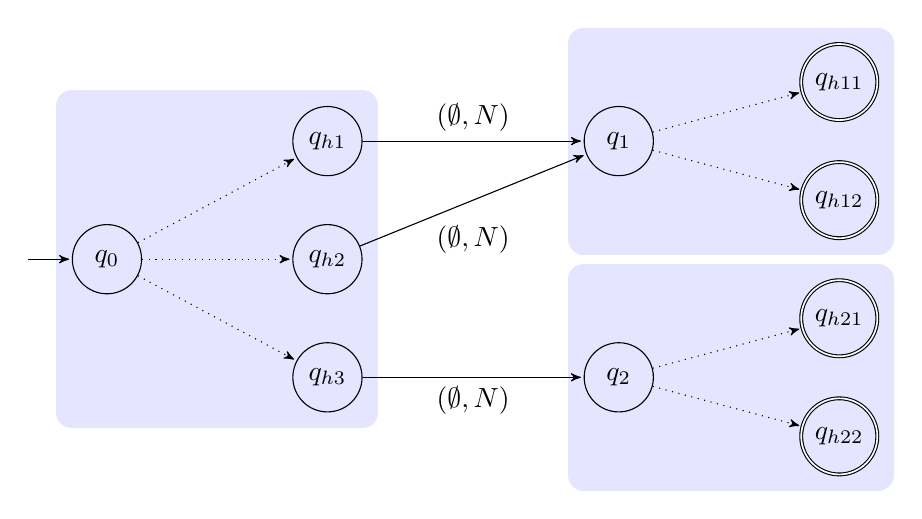
\begin{tikzpicture}[->,>=stealth',shorten >=1pt,auto,node distance=2.8cm]
    \begin{scope}
      % Machine M
      \node[state]          (M init)                                    {$q_0$};
      \node[state]          (M exit 1)  [right of=M init,yshift= 1.5cm] {$q_{h1}$};
      \node[state]          (M exit 2)  [right of=M init,yshift= 0.0cm] {$q_{h2}$};
      \node[state]          (M exit 3)  [right of=M init,yshift=-1.5cm] {$q_{h3}$};
      \path (M init)
      edge[dotted] (M exit 1)
      edge[dotted] (M exit 2)
      edge[dotted] (M exit 3);
      \path (M init) ++(-1.0,0) edge (M init);
    \end{scope}
    \begin{scope}[xshift=6.5cm]
      % Match-Machines
      \begin{scope}[yshift=1.5cm]
        % Accepting match machine
        \node[state]          (M 1 init)                                        {$q_1$};
        \node[state, double]  (M 1 exit 1)  [right of=M 1 init, yshift= 0.75cm]{$q_{h11}$};
        \node[state, double]  (M 1 exit 2)  [right of=M 1 init, yshift=-0.75cm] {$q_{h12}$};
        \path (M 1 init)
        edge[dotted] (M 1 exit 1)
        edge[dotted] (M 1 exit 2);
      \end{scope}
      \begin{scope}[yshift=-1.5cm]
        % Accepting match machine
        \node[state]          (M 2 init)                                        {$q_2$};
        \node[state, double]  (M 2 exit 1)  [right of=M 2 init, yshift= 0.75cm] {$q_{h21}$};
        \node[state, double]  (M 2 exit 2)  [right of=M 2 init, yshift=-0.75cm] {$q_{h22}$};
        \path (M 2 init)
        edge[dotted] (M 2 exit 1)
        edge[dotted] (M 2 exit 2);
      \end{scope}
    \end{scope}
    % Connecting edges
    \path
    (M exit 1) edge node[anchor=south] {$(\None, N)$} (M 1 init)
    (M exit 2) edge node[anchor=north,yshift=-0.2cm] {$(\None, N)$} (M 1 init)
    (M exit 3) edge node[anchor=north] {$(\None, N)$} (M 2 init);

    \begin{pgfonlayer}{background}
      \filldraw [line width=4mm,join=round,blue!10]
      (M   exit 1.north -| M   init.west) rectangle (M   exit 3.south -| M   exit 3.east)
      (M 1 exit 1.north -| M 1 init.west) rectangle (M 1 exit 2.south -| M 1 exit 2.east)
      (M 2 exit 1.north -| M 2 init.west) rectangle (M 2 exit 2.south -| M 2 exit 2.east);
    \end{pgfonlayer}
  \end{tikzpicture}

  \caption{Example for a match.  The left blue box stands for the initial machine.  After it reaches on of the terminal states $q_{h1}, \dots, q_{h3}$
    it continues its execution either in the right top machine or in the right bottom case machine.  The halting states of the match machines are
  exactly the halting states of the case-machines.}
  \label{fig:match-example}
\end{figure}

The idea of the \emph{match} operator is, to first execute a machine, and -- depending of the outcome of the execution -- continue the execution with
another machine.  To define this operator, the parametrised relational approach is in particular useful here.  This idea is illustrated in Figure
\ref{fig:match-example}.

First we fix a machine $M$ with a partition function $p$ into a finite type $F$.
We furthermore fix an $F$-indexed sequence of machines $M_f$ with partitions $p_f$ into another finite type $F'$.
All machines must have the same alphabet ($\Sigma$) and number of tapes ($n$).

The states of the machine are either states of $M$ or states of a machine $M_f$:
$$Q_{match} := Q_M + \setMap{(f, q_f)}{f \in F \land q_f \in Q_f}.$$
The initial state is $init_{match} := init_M$.  Now we define the new $\gamma_{match}$.
\begin{alignat*}{2}
  \gamma_{match}(q \in Q_M, tapes) &:=
  \begin{cases}
    \gamma_{M}(q, tapes) & h_M(q) = \false \\
    (q_{0, p(q)}, (\None, N)^n) & h_M(q) = \true
  \end{cases} \\
  \gamma_{match}(q \in Q_f, tapes) &:= \gamma_{M_f}(q, tapes)
\end{alignat*}

The halting states are exactly the halting states of each $M_f$:
\begin{alignat*}{2}
  h_{match}(q \in Q_M) &:= \false \\
  h_{match}(q \in Q_f) &:= h_{M_f}(q)
\end{alignat*}

Now we want to specify the semantics of the match machine and give a quick overview about the verification.

First we have to specify the partition function $p_{match} \from Q_{match} \to F'$:
\begin{alignat*}{2}
  p_{match}(q \in Q_M) &:= p_{p~q} (init_{p~q}) \\
  p_{match}(q \in Q_f) &:= p_f(q)
\end{alignat*}
Note that the machine can not halt in an inner state of $M$, thus the first case of the definition of $p_{match}$ is over-specified.

Now we assume the correctness relation $R \subseteq \Tapes{n} \times (F \times \Tapes{n})$ of $M$ and a family of relations
$R_f \subseteq \Tapes{n} \times (F' \times \Tapes{n})$ for each case-machine $M_f$.

We can show that if $M$ realises $R$ and each $M_f$ realises $R_r$ (either weekly or strongly), then $M_{match}$ realises
$$R_{match} := \bigcup_{f \in F} (R \at f) \circ R_f.$$
Note that this relation is a quite intuitive and a precise description of the behaviour of our defined operator:  First $M$ terminates into a state
that corresponds to some $f$ and then executes the machine $M_f$.

The correctness proof is quiet tedious.  The key idea is to first abstract from machines and argue about $loop$.  We come up with the following
lemmas:

\begin{lemma}[Lift loop]
  \label{lem:loop-lift}
  Let $A, B$ be types and $k \in \Nat$, $lift \from A \to B, f \from A \to A$, $g \from B \to B$, $hlift \from B \to \Bool$ and $c_1, c_2 \in A$.
  If $\forall~x \in X,~hlift (lift x) = h x)$ and $\forall x\in X,~ h~x = \false \rightarrow lift~(f~x) = g~(lift~x)$ and
  $loop~k~f~h~c_1 = \Some{c_2}$, then $loop~k~g~hlift~(lift~c_1) = \Some{lift~c_2}$.
\end{lemma}

\begin{lemma}[Merge loop]
  \label{lem:loop-merge}
  Let $A$ be a type, $f \from A \to A$ a step function, $p, q \from A \to \Bool$ halting functions, $k_1, k_2$ counts and $a_1, a_2, a_3 \in A$.
  If $\forall~a \in A,~p~a = \false \rightarrow q~b = \false$, $loop~k_1~f~p~a_1 = \Some{a_2}$, and $loop~k_2~f~q~a_2 = \Some{a_3}$, then
  $loop~(k_1 + k_2)~f~q~a_1 = \Some{a_3}$.
\end{lemma}

\begin{lemma}[Split loop]
  \label{lem:loop-split}
  Let $A$ be a type, $f \from A \to A$ a step function, $p, q \from A \to \Bool$ halting functions, and $a_1, a_3 \in A$.
  If $\forall~a \in A,~p~a = \false \rightarrow q~b = \false$ and $loop~k~f~q~a_1 = \Some{a_3}$, then there exists a step counts $k_1, k_2$ and an
  intermediate value $a_2 \in A$, such that $loop~k_1~f~p~a_1 = \Some{a_2}$ and $loop~k_2~f~q~a_2 = \Some{a_3}$, and $k = k_1 + k_2$.
\end{lemma}

\begin{lemma}[Unlift loop]
  Let $X, Y$ be types and $f \from X \to X$, $f' \from Y \to Y$ step functions, and $p \from X \to \Bool$, $q \from Y \to \Bool$ halting functions.
  We assume $\forall~a,a' \in X,~unlift~a = \Some{a'} \rightarrow p'~a' = \false \rightarrow unlift~(f~a) = \Some{f' a'}$.
  Furthermore we assume $\forall~a,a' \in A,~unlift~a = \Some{a'} \rightarrow p~a = p'~a'$.
  If $unlift~a = \Some{a'}$ and $loop~i~f~p~a = \Some{x}$, then
  there exists a $y' \in Y$, such that $loop~i~f'~p'~a' = \Some{y'} = unlift~x$.
\end{lemma}

Using this lemmas we can prove the correctness statement for the $match$-machine:
\begin{lemma}[Correctness of $match$]
  If $M \vDash_p R$ and for each $f \in F$, $M_f \vDash_{p_f} R_r$, then
  $$\mmatch~M~(M_f, p_f) \vDash \bigcup_{f \in F} (R \at f) \circ R_f.$$
\end{lemma}

Now that we have a match combinator, sequential composition and boolean if can be reduced to it, by arguing that sequential composition is just a
trivial matching from any states of $M_1$ to $M_2$, and a boolean if amounts to matching over a boolean value:

\begin{definition}[Sequential composition]
  \label{def:seq}
  Let $M_1, M_2$ be a $n$-tape machines over $\Sigma$ with the partitioning function $p_1 \from Q_1 \to F_1$ and $p_2 \from Q_2 \to F_2$,
  respectively.  Then we define the \emph{sequential composition} of $M_1$ and $M_2$:
  $$M_1 \mseq M_2 := \mmatch~(M_1, p_1)~(\lam y (M_2, p_2))$$
\end{definition}

\begin{corollary}[Correctness of sequential composition]
  \label{lem:seq}
  If $M_1 \vDash R_1$ and $M_2 \vDash R_2$, then $M_1 \mseq M_2 \vDash R_1 \circ hideParam(R_2)$.
\end{corollary}

\begin{definition}[Boolean if]
  \label{def:if}
  Let $M_1, M_2, M_3$ be a $n$-tape Turing machines over $\Sigma$.
  Let $p_1 \from Q_1 \to \Bool$ and $p_2 \from Q_2 \to F', p_3 \from Q_3 \to F'$ be partitioning functions.
  Then we define \emph{boolean if}:
  $$\mif{M_1}{M_2}{M_3} := match~(M_1, p_1) \left(\lam b \begin{cases} (M_2; p_2) & b = \true \\ (M_3; p_3) & b = \false \end{cases} \right)$$
\end{definition}

\begin{corollary}[Correctness of boolean if]
  \label{lem:if}
  If $M_1 \vDash R_1$ and $M_2 \vDash R_2$ and $M_3 \vDash R_3$, then
  $\mif{M_1}{M_2}{M_3} \vDash (R_1 \at \true) \circ R_2 \cup (R_1 \at \false) \circ R_3$.
\end{corollary}


\subsection{While}

\begin{figure}
  \center
  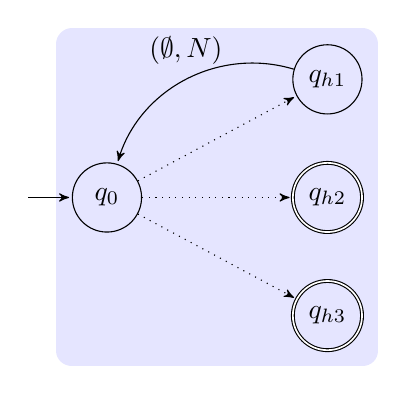
\begin{tikzpicture}[->,>=stealth',shorten >=1pt,auto,node distance=2.8cm,bend angle=45]
    \begin{scope}
      % Machine M
      \node[state]          (M init)                                    {$q_0$};
      \node[state]          (M exit 1)  [right of=M init,yshift= 1.5cm] {$q_{h1}$};
      \node[state, double]  (M exit 2)  [right of=M init,yshift= 0.0cm] {$q_{h2}$};
      \node[state, double]  (M exit 3)  [right of=M init,yshift=-1.5cm] {$q_{h3}$};
      \path (M init)
      edge[dotted]          (M exit 1)
      edge[dotted]  (M exit 2)
      edge[dotted]  (M exit 3);
      \path (M init) ++(-1.0,0) edge (M init);
      \path (M exit 1) edge[bend right] node[anchor=south,yshift=0.2em] {$(\None, N)$} (M init);
    \end{scope}

    \begin{pgfonlayer}{background}
      \filldraw [line width=4mm,join=round,blue!10]
      (M   exit 1.north -| M   init.west) rectangle (M   exit 3.south -| M   exit 3.east);
    \end{pgfonlayer}
  \end{tikzpicture}
  \caption{Example for a do-while-loop.  When the machine reaches the state $q_{h1}$ it restarts.  It holds in the final states $q_{h2}$ and $q_{h3}$.}
  \label{fig:while-example}
\end{figure}

The \emph{while} operator implements a \emph{do-while-loop}.  The loop condition, however, is encoded through the boolean partition
function of the terminal states:  We insert transitions from the ``positive'' halting states.  This idea is depicted in Figure
\ref{fig:while-example}.

We define the while-machine formally.  Let $M$ be a machine with a boolean partition function $p \from Q \to \Bool$.  The transition function is
$$\gamma_{while} (q, tapes) :=
  \begin{cases}
    (q_0, (\None, N)^n)   & h(q) = \true \land p(q) = true \\
    \gamma(q, tapes)      & \txt{else}
  \end{cases} $$
The halting states are the ``negative'' halting states of $M$:
$$halt_{while}(q) := halt_M(q) \land p(q) = \false.$$

We can describe the semantics of the while-machine with help of the Kleene star:

\begin{lemma}[Semantics of the while-machine]
  If $M \vDash R$, then $\mwhile{M} \vDash_{\lam x \unit} \left(R \at \true \right)^* \circ ignoreParam \left(R \at \false \right)$.
\end{lemma}

The correctness proof is similar to the correctness proof of the $\mmatch$ machine.

\section{Machine transformations}
\label{sec:transformations}

Using the operators above, we can build and verify small machines with ease.  However, to compose machines, they have to agree in their alphabet and in
their number of tapes.  Because this not always the case, we introduce new operators, that ``enlarge'' a given machine by either introducing new tapes
or by ``translating'' alphabets.


% FIXME: called n,m-lift in Coq.  This is *wrong*!

\subsection{\texorpdfstring{$m,n$}{m,n}-lift}

% TODO: Better graphic
\begin{figure}
  \center
  % \begin{tikzpicture}
  %   % \draw[very thick] (0,1) -- (0,2);
  %   % \draw[very thick] (3,3) -- (3,0);
  %   \draw[<->] (0,2) -- (3,2);
  %   \draw[<->] (0,1) -- (3,0);
  %   % \foreach \y in {0,1}
  %   %   \draw[yshift=-\y cm] (-2pt,2) -- (2pt,2) node[anchor=east] {$\y$};;
  %   % \foreach \y in {0,1,2,3}
  %   %   \draw[yshift=-\y cm] (3cm-2pt,3) -- (3cm+2pt,3) node[anchor=west] {$\y$};;
  % \end{tikzpicture}
  \begin{tikzpicture}
    \begin{scope}
      \node(a0)[yshift=-0 cm]  {$0$};
      \node(a1)[yshift=-1 cm]  {$1$};
      \node(a2)[yshift=-2 cm]  {$2$};
    \end{scope}
    \begin{scope}[xshift=4cm, yshift=0cm]
      \node(b0)[yshift=-0 cm] {$0$};
      \node(b1)[yshift=-1 cm] {$1$};
      \node(b2)[yshift=-2 cm] {$2$};
      \node(b3)[yshift=-3 cm] {$3$};
      \node(b4)[yshift=-4 cm] {$4$};
    \end{scope}
    \begin{scope}[xshift=5cm, yshift=-3cm]
      \node(none)             {$\None$};
    \end{scope}
    \path (a0) edge[<->] (b1);
    \path (a1) edge[<->] (b0);
    \path (a2) edge[<->] (b3);
    \path (b2) edge[-> ] (none);
    \path (b4) edge[-> ] (none);
  \end{tikzpicture}
  \caption{An example for a retract between tape indexes, for $m=2$ and $m=4$.  The arrows from the left to the right correspond to the
  function $f$. The function $g$ maps $1$ back to $\Some{0}$ and $3$ to $\Some{2}$, all other values are mapped to $\None$.}
  \label{fig:m-n-lift-example-mapping}
\end{figure}

The most of our machines do really only work on one or two tapes, but they have to be embedded into ``bigger'' machines with more tapes.  There are
two possible routes to follow:  One way to solve this problem could be to define all these machines as $n$-tape machines and give them the
tape-indexes on which the machine should operate.  We could also define those machines as e.g. two-tapes machines and then define an ``lift''
operation that can automatically build an arbitrary big machine that only operates on two of its tapes and emulates the behaviour of the smaller
machine.

However, the first approach seems unsatisfying, because definition and verification of small Turing machines is easier.  We don't want to struggle
every time with this, when we define a new machine.

Therefore we have invented the $m,n$-lift. For $n \ge m$, given a $m$-tape Turing machine it yields a $n$-tape Turing machine that has exactly the
same behaviour but ignores the other $n-m$ tapes.  The operator takes a retract from $m$-tape indexes to $n$-tape indexes.  This mapping has to be
injective, because the behaviour of a tape can not be ``duplicated'', because tapes can behave different in different contexts.  We need the inversion
function of the retract to translate the indexes back in the transition function $\gamma$.

For example, with $m=3$ and $n=5$ and we can  map the tape $0$ to the tape $1$, tape $1$ to tape $0$, and tape $2$ to tape $3$, as depicted in Figure
\ref{fig:m-n-lift-example-mapping}.


% XXX Coq code uses index vectors.  Are retracts better in practice?
Let $M$ be a $m$-tape Turing machine over $\Sigma$.  Let $n \ge m$.  Let $(f, g) \from \Fin_m \hookrightarrow \Fin_n$ be a retract.

For the definition and verification of the $m,n$-lift we need two functions:  First we need the polymorph function
$inject \from X^m \to X^n \to X^n$, that inserts all values in the image of $f$ from $m$-vector into the $n$-vector:
\begin{align*}
  inject~xs~ys := tabulate \left(\lam i
    \begin{cases}
      xs[j]   & g(i) = \Some{j} \\
      ys[i]   & g(i) = \None
    \end{cases}
  \right)
\end{align*}
The second function we need is $reorder \from X^n \to X^m$, that selects the values of the indexes in the image of $f$:
$$reorder~ys := tabulate \left( \lam j ys[j] \right)$$

The states, initial state, final states, the alphabet, and the state partitioning of the lift-machine are inherited from $M$.  Using these two
functions we can define the transition function $\gamma$:
\begin{alignat*}{3}
  &\gamma (q, sym)  &~:=~& \mlet {(q', act) := \gamma_M(q, reorder~sym)}{\\
  &                 &~  ~& (q',~inject~act~(\None, N)^n)}
\end{alignat*}

\begin{definition}[Relational $m,n$-lift]
  \label{def:m,n-rellift}
  For $R \subseteq \Tapes{n} \times (F \times \Tapes{n})$
  $$RLift_{m,n}(R) := \setMap{(input, (y, output))}{(reorder~input, (y, reorder~output)) \in R}$$
\end{definition}

\begin{lemma}[Correctness of the $m,n$-lift]
  \label{lem:m,n-correctness}
  Let $R \subseteq \Tapes{n} \times (F \times \Tapes{n})$ be a parametrised relation.  If $M \vDash R$, then $Lift_{m,n} \vDash RLift_{m.n}(R)$.
\end{lemma}
\begin{proof}
  This can be shown by induction, first over the number of steps, then over $m \in \Nat$.
\end{proof}


% XXX Termination not yet shown in Coq
\subsection{\texorpdfstring{$\Sigma,\Tau$}{Sigma,Tau}-Lift}

\begin{figure}
  \center
  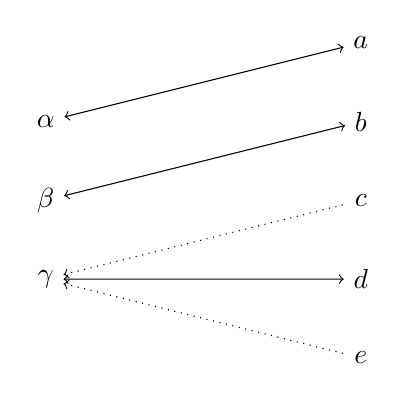
\begin{tikzpicture}
    \begin{scope}
      % Symbols of $\Sigma$
      % FIXME This loop does not work!
      % \foreach \x / \y in {0 / \alpha, 1 / \beta, 2 / \gamma}
      %   \node(sigma\x)[yshift=-\x cm] {$\y$};;
      \node(alpha)[yshift=-0 cm] {$\alpha$};
      \node(beta) [yshift=-1 cm] {$\beta$};
      \node(gamma)[yshift=-2 cm] {$\gamma$};
    \end{scope}
    \begin{scope}[xshift=4cm, yshift=1cm]
      % Symbols of $\Tau$
      \node(a)[yshift=-0 cm] {$a$};
      \node(b)[yshift=-1 cm] {$b$};
      \node(c)[yshift=-2 cm] {$c$};
      \node(d)[yshift=-3 cm] {$d$};
      \node(e)[yshift=-4 cm] {$e$};
    \end{scope}
    \path (alpha) edge[<->] (a);
    \path (beta)  edge[<->] (b);
    \path (gamma) edge[<->] (d);
    \path (gamma) edge[<-, dotted] (c);
    \path (gamma) edge[<-, dotted] (e);
  \end{tikzpicture}
  \caption{An example for a retract plus default element between the alphabets $\Sigma = \setOf{\alpha, \beta, \gamma}$ and $\Tau =
  \setOf{a,b,c,d,e}$.  The symbols $c$ and $e$, that are not in the image of $f$, are implicitly mapped to $\gamma$, the default element in $\Sigma$.}
  \label{fig:sigma-tau-lift-example-mapping}
\end{figure}

Similarly to the $m,n$-Lift, the $\Sigma,\Tau$-Lift extends the alphabet of a Turing machine.  The operator gets a retract
$(f,g) \from \Sigma \hookrightarrow \Tau$.  However we also have to give an symbol $default \in \Sigma$, for the symbols in $\Tau$ that can not be mapped back to
$\Sigma$.  This idea is illustrated in Figure \ref{fig:sigma-tau-lift-example-mapping}.

Let $M$ be a $n$-tape Turing machine over $\Sigma$.  The alphabet of the lift-machine $\Tau$.  The states, initial states, and the final states, and
the partitioning are inherited from $M$.  To define the transition function, we have to define some functions again.  First need a function that
applies a translation function to a tape:
\begin{definition}[Map tapes]
  We define the higher-order function
  $map\_tape \from (\Tau \to \Sigma) \to \Tape_\Sigma \to \Tape_\Tau$
  that applies $map$ to the symbols of a tape.
  \begin{alignat*}{2}
    map\_tape&~g~(\tape{})                  &&:= \tape{} \\
    map\_tape&~g~(\tape{\tapePointer{} r~R})   &&:= \tape{\tapePointer{}~(g~r)~(map~g~R)} \\
    map\_tape&~g~(\tape{L \tapePointer{m}~R})  &&:= \tape{(map~g~L) \tapePointer{(g~m)} (map~g~R)} \\
    map\_tape&~g~(\tape{L~l \tapePointer{}})   &&:= \tape{(map~g~L)~(g~l) \tapePointer{}}
  \end{alignat*}
\end{definition}

Now we need a helper function that translates actions:
\begin{definition}[Translate action]
  \label{def:translate-action}
  Let $\Sigma$ and $\Tau$ be alphabets and $f \from \Sigma \to \Tau$ a translation function.  We define the function
  $$translate\_act(w, m) \from \Opt(\Sigma) \times Move \to \Opt(\Tau) \times Move$$
  \begin{align*}
    translate\_act (w, m) :=
    \begin{cases}
      (g(w'), m)  & w = \Some{w'} \\
      (\None, m)  & w = \None
    \end{cases}
  \end{align*}
\end{definition}

Then we can define the function $surject \from \Tau \to \Sigma$, that is $g$ extended by $default$:
\begin{align*}
  surject~\tau :=
  \begin{cases}
    s         & g~\tau = \Some{s} \\
    default   & g~\tau = \None
  \end{cases}
\end{align*}

Furthermore we define $surject\_tape(tape) := map\_tape~surject~t$ and $surject\_tapes(tapes) := map~surject\_tape~tapes$.  Now we can finally define
the transition function $\gamma$ of the $\Sigma,\Tau$-lift:
\begin{alignat*}{3}
  &\gamma (q, sym)  &~:=~& \mlet {(q', acts) := \gamma_M(q, map~(translate\_act~surject)~sym)}{\\
  &                 &~  ~& (q', map~(translate\_act~f)~acts)}
\end{alignat*}

Now, that we have defined the $\Sigma,\Tau$-lift, we look at how we must transform the relation.
\begin{definition}[Relational $\Sigma,\Tau$-lift]
  \label{def:sigma,tau-rellift}
  For $R \subseteq \Tapes{n} \times (F \times \Tapes{n})$
  $$RLift_{\Sigma,\Tau} := \setMap{(input, (y, output))}{(surject\_tapes~input, (y, surject\_tapes~output)) \in R}$$
\end{definition}

\begin{lemma}[Correctness of the $\Sigma,\Tau$-lift]
  \label{lem:sigma,tau-correctness}
  Let $R \subseteq \Tapes{n} \times (F \times \Tapes{n})$ be a parametrised relation.  If $M \vDash R$, then
  $Lift_{\Sigma,\Tau} \vDash RLift_{\Sigma, \Tau}(R)$.
\end{lemma}
\begin{proof}
  This can be shown by induction, first over the number of steps, then over $m \in \Nat$.
\end{proof}

\section{Compound machines}

% TODO: Implement/present compound machines
TODO: Implement/present compound machines

\subsection{Write string}

One other operation that we need is writing a certain string on a tape instead of only a single symbol.  We give a movement direction $D$ as
parameter and define this machine by recursion over the string:
\begin{alignat*}{3}
  Write\_String&~\nil       ~&& D := Nop \\
  Write\_String&~(e \cons l)~&& D := Write~e \mseq Move~D \mseq Write\_String~l
\end{alignat*}


\section{Encoding types}
\label{sec:encode}

To approach an interpreter for $\lambda$-terms, we have to define encodings for all occurring data types.
We define encodable types as a type class parametrised by the alphabet.

\begin{definition}[Codeable type]
  \label{def:code}
  A type $X$ is \emph{encodable} in an alphabet $\Sigma$, if there exists an \emph{encoding function}
  $encode \from X \to \List(\Sigma)$ with the property:
  \begin{multline*}
    \forall~v_1,v_2 \in X,~r_1,r_2 \in \List(\Sigma), \\
    encode(x) \app r_1 = encode(v_2) \app r_2 \Rightarrow
    v_1 = v_2 \land r_1 = r_2.
  \end{multline*}
\end{definition}
Note that this property implies injectivity of the encoding function.  Because we can not make tapes smaller, the machine that interacts with encoded
values must know where the string ends.  Therefore injectivity of the encoding function alone is not enough.

Our Coq development provides a library of encoding functions for typical types, for example:  $\Unit$, $\bot$, $\Opt(X)$, $X+Y$, $X \times Y$, $\List(X)$
and $\Nat$.  Note that each type can be encoded on different alphabets.  For example we can encode every finite type $F$ to the alphabet $F$ itself.

\begin{example}[Encoding basic types]
  \label{ex:bacic-code}
  $\Unit$ and $\bot$ are encoded on the empty alphabet, while every finite type $F$ encodes itself:
  \begin{alignat*}{3}
    encode&_F    &&~(f \in F)         &&:= [f] \\
    encode&_\bot &&~(devil \in \bot)  &&:= [] \\
    encode&_\Unit&&~(\unit \in \Unit) &&:= [] \\
  \end{alignat*}
\end{example}

To encode more complex types we need a mechanism to extend an alphabet.
\begin{lemma}[Alphabet mapping]
  \label{lem:code-map}
  Let $X$ be a type and $\Sigma, \Tau$ be alphabets.
  Let $encode \from X \to \List(\Sigma)$ be an encoding function for $X$ on $\Sigma$.
  Let $(f,g) \from \Sigma \hookrightarrow \Tau$ be a tight retract.
  Then we can define an encoding function $encode_{\Sigma \hookrightarrow \Tau} \from X \to \List(\Tau)$.
\end{lemma}

\begin{proof}
  We define the new encoding function:
  $$encode_{\Sigma \hookrightarrow \Tau}(x) := map~f~(encode~x).$$
  To show that this is a valid encoding function, it suffices to show the following lemma:
  \begin{multline*}
    \forall~v_1,v_2 \in X,~\forall~r_1, r_2 \in \List(\Sigma),~\forall~R_1, R_2 \in \List(\Tau),\\
    map~f~(encode~v_1 \app r_1) \app R_1 = map~(encode~v_2 \app r_2) \app R_2 \Rightarrow \\
    v_1 = v_1 \land map~f~r_1 \app R_1 = map~f~r_2 \app R_2.
  \end{multline*}
  This can be shown by double-induction over $R_1, R_2 \in \List(\Tau)^2$.
\end{proof}


\begin{corollary}[Extend alphabets]
  \label{lem:extend-alphabet}
  Let $X, Y$ be types encodable over $\Sigma$ and $\Tau$, respectively.
  Using Lemma \ref{lem:code-map} we can build new encoding functions:
  \begin{alignat*}{2}
    encode_{\Sigma \hookrightarrow \Sigma + \Tau} &\from X \to \List(\Sigma + \Tau) \\
    encode_{\Tau   \hookrightarrow \Sigma + \Tau} &\from Y \to \List(\Sigma + \Tau) \\
    encode_{\Sigma \hookrightarrow \Opt(\Sigma)}  &\from X \to \List(\Opt(\Sigma)) \\
    encode_{\Sigma + \bot \hookrightarrow \Sigma} &\from X \to \List(\Sigma).
  \end{alignat*}
\end{corollary}

Using Corollary \ref{lem:extend-alphabet} we can construct encoding functions for compound types:
\begin{corollary}[Encoding compound types]
  \label{lem:code-compound}
  Let $X, Y$ be types encodable over $\Sigma$ and $\Tau$, respectively.
  Then the following functions are encoding functions:
  \begin{alignat*}{2}
    encode_{X+Y}&(x)             &&:= \false                 \cons encode_{\Sigma \hookrightarrow \Sigma + \Tau}(x) \\
    encode_{X+Y}&(y)             &&:= \true \hspace{0.15em} \cons encode_{\Tau   \hookrightarrow \Sigma + \Tau}(y) \\
    encode_{\List(X)}& (\nil)    &&:= \false \\
    enocde_{\List(X)}& (x :: xs) &&:= \true \hspace{0.15em} \cons encode_{\Sigma \hookrightarrow \Bool + \Sigma}(x) \app
                                      encode_{\List(X) \hookrightarrow \Bool + \Sigma}(xs)
  \end{alignat*}
\end{corollary}

We will now see how we can encode tuples.  If we have types $X$ and $Y$ that are encodable over the same alphabet $\Sigma$, it is easy:
$$encode(x,y) := encode(x) \app encode(y).$$
However, if we encode $X$ over $\Sigma$ and $\Tau$, we first have to map the alphabets to $\Sigma + \Tau$:
$$encode(x,y) := encode_{\Sigma \hookrightarrow \Sigma + \Tau}(x) ++ encode_{\Tau \hookrightarrow \Sigma + \Tau}(y).$$

We want to reduce the encoding of $\Nat$ to the encoding of $\List(\Unit)$.
\begin{lemma}[Code reducing]
  \label{lem:code-reduce}
  Let $Y$ be a type encodable over $\Sigma$.
  Let $f \from X \to Y$ be an injective function.
  Then $encode(x) := encode(f(x))$ is an encoding function for $X$ on $\Sigma$.
\end{lemma}
\begin{corollary}
  Using lemma \ref{lem:code-reduce} we can derive following encoding functions:
  \begin{alignat*}{4}
    encode&_\Nat      &&\from \Nat    &&\to \List(\Bool) \\
    encode&_{\Opt(X)} &&\from \Opt(X) &&\to \List(\Bool + \Sigma).
  \end{alignat*}
\end{corollary}


\section{Approaching an interpreter}

Finally we want to define a notion that a Turing machine \emph{computes} a function.  Therefore we need a predicate $encodes \subseteq Tape \times X$
for an encodable type $X$.

We have several possibilities to define such a predicate.  The first possibility is that the current string on the tape encodes the value:
$$encodes(tape, x) := encode_X(x) = tape\_to\_string(tape).$$
This is not a good definition: Since it is impossible to remove symbols from a tape, we can not ``decrease'' $x$ (that means that the encoding of
$x$ gets smaller).

To fix this problem, we can define the predicate in this way:
$$encodes(tape, x) := \exists~rest,~encode_X(x) \app rest = tape\_to\_string(tape).$$
However, one problem remains:  If a machine is supposed to only remove the first symbol of the encoding, it would have to shift the whole tape
content.

% XXX This has yet to be implemented.
We can solve this issues by introducing a $\mathbf{start}$ and a $\mathbf{end}$ symbol (using Corollary \ref{lem:extend-alphabet}):
\begin{multline*}
  encodes(tape,x) := \exists!~r_1,r_2,~\\
  r_1 \app [\mathbf{start}] \app encode_{X \hookrightarrow X + \Bool}(x) \app [\mathbf{end}] \app r_2 = \\
  tape\_to\_string(tape).
\end{multline*}

Now it is possible to define computation of a function:
\begin{definition}[Computation of a function]
  \label{def:computes}
  Let $X, Y$ be encodable types over $\Sigma$.  A machine $M$ \emph{computes} a function $f \from X \to Y$ on tape number $i < n$, if
  $$M \vDash \setMap{(input, (y, output))}{\forall~x \in X,~ encodes(input[i], x) \Rightarrow encodes(output[i], f(x))}.$$
\end{definition}

We can already show that functional computation is compositive:
\begin{lemma}[Compose functions]
  \label{lem:computes-composes}
  Let $X, Y, Z$ be encodable types over $\Sigma$.  If $M_1$ and $M_2$ are $n$-tape Turing machines over $\Sigma$ and $M_1$ computes
  $f \from X \to Y$ on tape number $i$ and $M_2$ computes $g \from Y \to Z$, then $M_1 \mseq M_2$ computes $f \circ g \from X \to Z$.
\end{lemma}
\begin{proof}
  Follows with the correctness statement of composition, see Lemma \ref{lem:seq}.
\end{proof}

Note that in Lemma \ref{lem:computes-composes} the two machines have to compute the functions on the same tape.  We can get rid of this restriction
using the following Lemma:
\begin{lemma}[Compute function on different tape]
  If there exists a machine $M$ that computes a function $f$ on tape $i$ then there exists a machine that computes $f$ on any tape $j$.
\end{lemma}
\begin{proof}
  Using the $n,m$-Lift we swap the tapes $i$ and $j$.
\end{proof}

% XXX This has yet to be implemented
The next big milestone is to implement \emph{recursive functions}.  For example, if we want to implement a tail-recursive function over lists, the
upper-most machine is an $while$.  Inside the while-loop we use the $match$-operator using the $read$ machine to check the first symbol, that is
$\true$ for a non-empty list and $\false$ for $\nil$.  If the recursion terminates in one of these cases, the corresponding $case$-machine will
terminate in a state that corresponds to $\false$.  Otherwise the wile-loop will be repeated.

\end{document}

% TODO Profread

%%% Local Variables:
%%% mode: latex
%%% TeX-master: t
%%% End:
% vim: ts=2 sts=2 sw=2 expandtab textwidth=150
